\documentclass[11pt]{exam}
\usepackage[margin=1in]{geometry}
\pagestyle{plain}
\usepackage{amsmath,amsfonts,amssymb,amsthm,enumerate}
\usepackage{multicol}
\usepackage[]{graphicx}
\usepackage{hyperref}
\usepackage{tikz}
\usepackage{pgfplots}
\usepackage{subfigure}
\usepackage[final]{pdfpages}

\everymath{\displaystyle}

\addtolength{\footskip}{2\baselineskip} % to lower the page numbers
\title{\vspace{-0.5in} Math 115 \\ Worksheet Section 5.4}
\date{}


% \theoremstyle{definition}
% \newtheorem{problem}{Problem}
\renewcommand{\questionlabel}{\textbf{Problem~\thequestion.}}
%\printanswers

\begin{document}
\maketitle
\vspace{-0.75in}
\begin{questions}
  \question Find each integral, given that $\int_a^b f(x) dx = 8, \int_a^b (f(x))^2 dx = 12,$ and $\int_a^b g(t) dt= 2.$  
    \begin{parts}
    \part $\int_b^a (f(x))^2 dx - \left(\int_a^b f(x) dx\right)^2$
    \part $\int_a^b (c_1 g(x) +(c_2f(x))^2) dx$
    \part $\int_{a+5}^{b+5} f(x-5) dx$
    \end{parts}
    \begin{solution}
      \begin{enumerate}[(a)]
      \item \[
          \int_b^a (f(x))^2 dx - \left(\int_a^b f(x) dx\right)^2 = -12-(8)^2 = -76
        \] 
      \item \[
          \int_a^b (c_1 g(x) +(c_2f(x))^2 dx = c_1 \int_a^b g(x) dx +
          c_2^2 \int_a^b (f(x))^2 dx = 2 c_1 + 12 c_2^2
        \]
      \item \[
          \int_{a+5}^{b+5} f(x-5) dx = \int_a^b f(x) dx = 8
        \]
      \end{enumerate}
    \end{solution}
  \question If $f(x)$ is an odd function and $\int_{-2}^3 f(x) dx = 30$, find $\int_2^3 f(x) dx$.
    \begin{solution}
      Remember that an odd function satisfies \(f(-x) =
      -f(x)\) and so \(\int_{-a}^a f(x) dx = 0\) for any \(a \geq 0\). Thus, \[
        30 = \int_{-2}^3 f(x) dx = \int_{-2}^2 f(x) dx + \int_2^3 f(x)
        dx = \int_2^3 f(x) dx
      \]
    \end{solution}
  \question Without computation, show that $2 \leq \int_0^2
    \sqrt{1+x^3} dx \leq 6$.  \textit{Hint: carefully draw a graph}. 
    \begin{solution}
      First, we notice that \(f(x) = \sqrt{1+x^3}\) is an increasing function.
      So we can check that \(\sqrt{1+x^3} \leq 3\) on the entirety of
      \([0,2]\) by simply plugging in \(x=2\) to get \(\sqrt{1+2^3} =
      3\). Similarly, \(\sqrt{1+x^3} 
      \geq 1\) on \([0,2]\) since \(\sqrt{1+0^3} = 1\). Thus,
      \begin{align*}
        1 \leq \sqrt{1+x^3} \leq 3
        & \implies \int_0^2 1 dx \leq \int_0^2 \sqrt{1+x^3} dx \leq
          \int_0^2 3 dx \\
        & \implies 2 \leq \int_0^2 \sqrt{1+x^3} dx \leq 6
      \end{align*}
    \end{solution}
  \question Without computation, explain why both of the following statements must be false.
 $$(a) \int_{-2}^{-1} e^{x^2} dx = -3  \quad \quad (b) \int_{-1}^1 \bigg|  \frac{\cos(x+2)}{1+\tan^2 x}\bigg| dx = 0$$
 \begin{solution}
   \begin{enumerate}[(a)]
   \item \(e^{x^2}\) is always positive, so its graph always lies
     above the \(x\)-axis. Therefore, for any \(a \leq b\), it must be
     that \[
       \int_a^b e^{x^2} dx \geq 0
     \]
   \item Similar to part (a), the graph must always lie above the
     \(x\)-axis, so the only way for the integral to be \(0\) is if
     the function were always equal to 0 between \(-1\) and \(1\). 
     This is not possible since \(\cos(-1+2) = \cos(1) \neq
     0\).
   \end{enumerate}
 \end{solution}
\question
  \begin{parts}
  \part Let \(s(t)\) be the position function of a particle and let
    \(v(t)\) be its velocity. Give a formula for the average
    velocity of the particle from \(t=a\) to \(t=b\) in terms of
    \(s(t)\) and give another formula in terms of \(v(t)\).
    \vspace{0.75in}
  \part For any function \(f(x)\), what is the average value of the
    function from \(x=a\) to \(x=b\)?
    \vspace{0.5in}
  \end{parts}
  \begin{solution}
    \begin{enumerate}[(a)]
    \item Average velocity from \(t=a\) to \(t=b\) is both
      \(\frac{s(b)-s(a)}{b-a}\) and also
      \(\frac{1}{b-a} \int_a^b v(t) dt\).
    \item The average value of any function \(f(x)\) from \(x=a\) to
      \(x=b\) is given by \[
        \frac{1}{b-a} \int_a^b f(x) dx
      \]
    \end{enumerate}
  \end{solution}
  \question A function \(f\) is graphed below
    \begin{multicols}{2}
      \begin{parts}
      \part Use the figure to find \(\int_1^6 f(x) dx\)
      \part What is the average value of \(f\) on \([1,6]\)?
      \end{parts}
      \columnbreak
      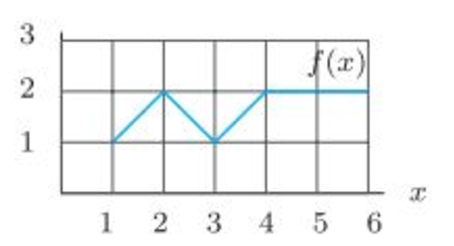
\includegraphics[scale=0.8]{graph_f}
    \end{multicols}
    \begin{solution}
      \begin{enumerate}[(a)]
      \item \(\frac{17}{2}\)
      \item The average value of \(f\) on \([1,6]\) is \[
\frac{1}{6-1} \int_1^6 f(x) dx = \frac{1}{5} \cdot \frac{17}{2} = 1.7
        \]
      \end{enumerate}
    \end{solution}
  \question If the average value of $f$ on the interval $2\leq x \leq 5$ is 4, find $\int_2^5(3f(x) + 2) dx$.
    \begin{solution}
      Since the average value of \(f\) on \([2,5]\) is \(4\), we
      know \[
        \frac{1}{5-2} \int_2^5 f(x) dx = 4 \implies \int_2^5 f(x) dx = 12
      \]
      Now, using our integration rules, we get \[
        \int_2^5 (3f(x)+2) dx = 3 \int_2^5 f(x) dx + \int_2^5 2 dx = 3
        \cdot 12 + 2(5-2) = 42
      \]
    \end{solution}
  \question The graph of \(f\) is given below. List the following
    quantities from least to greatest.
    \begin{minipage}{0.5\linewidth}
      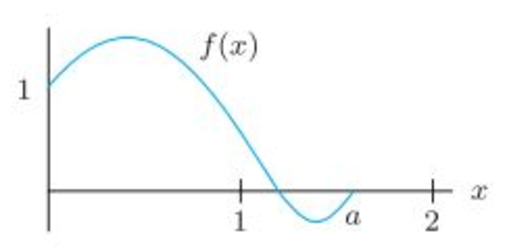
\includegraphics[scale=0.8]{graph_f2}
    \end{minipage}
    \begin{minipage}{0.5\linewidth}
      \begin{enumerate}[(I)]
      \item \(f'(1)\)
      \item The average value of \(f(x)\) on \(0 \leq x \leq a\).
      \item The average value of the rate of change of \(f(x)\), for
        \(0 \leq x \leq a\).
      \item \(\int_0^a f(x) dx\)
      \end{enumerate}
    \end{minipage}
    \begin{solution}
      We begin with some comparisons. Since \(a > 1\) and the signed
      area under the curve \(y=f(x)\) from \(0\) to \(a\) is positive, we get that \[
        0 < \text{Average value of }f\text{ on }[0,a] = \frac{1}{a-0}
       \int_0^a f(x) dx < \int_0^a f(x) dx
      \]
      We also can estimate \(\int_0^a f(x) dx \approx 1\).

      Next, we know that the average value of the rate of change is
      given by \[
        \frac{f(a)-f(0)}{a-0} = \frac{0-1}{a} = -\frac{1}{a} < 0
      \]
      and \(f'(1)\) is around the most negative \(f'(x)\) gets on
      \([0,a]\), so it must be that \(f'(1)\) is less than the average
      value of the rate of change of \(f(x)\) on \([0,a]\). Thus,
      putting it all together, we get
      \begin{center}
        I \(<\) III \(<\) II \(<\) IV
      \end{center}
    \end{solution}
  \question A bar of metal is cooling from 1000$^\circ$C to room temperature, $20^\circ$C.  The temperature, $H$, of the bar $t$ minutes after it starts cooling is given, in $^\circ$C, by $$H=20+980e^{-0.1t}.$$
\begin{enumerate}[(a)]
	\item Find the temperature of the bar at the end of one hour.
	\item Write an integral that gives the average value of the temperature over the first hour.
	\item Is your integral in (b) greater or smaller than the average of the temperatures at the beginning and the end of the hour?  Explain this in terms of the concavity of the graph of $H$.
\end{enumerate}
\begin{solution}
  \begin{enumerate}[(a)]
  \item \(H(1) = 20+980 e^{-0.1 (60)} = 20+980 e^{-6} \approx 22.4
    \, {}^\circ C\) 
  \item \[
      \frac{1}{60} \int_0^{60} H(t) dt
    \]
  \item The graph for \(H(t)\) is decreasing and concave up. The average of the
    temperature at \(t=0\) and the temperature at \(t=60\) will be
    the area under the secant line between \((0,H(0))\) and
    \((60,H(60))\) divided by \(60\) (convince yourself of
    this). Then, \(H(t)\) must lie below this line, so the integral in
    (b) must be less than the average of these two temperatures.
  \end{enumerate}
\end{solution}
\question (Fall 2016 Final Exam) % problem 5
The table below gives several values of a function $q(u)$ and its first and second derivatives. Assume that all of $q(u)$, $q'(u)$, and $q(u)$ are defined and continuous for all real numbers u.	
\begin{center}
  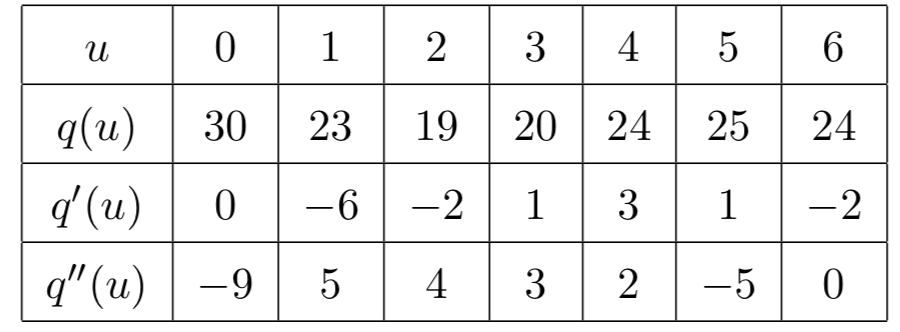
\includegraphics[scale=0.5]{tableq}
\end{center}
Compute each of the following. Do not give approximations. If it is not possible to find the value exactly, write not possible.
\begin{enumerate}[(a)]
	\item Compute $\displaystyle\int_5^2 q''(t) \, dt$.
	\item Suppose $q(u)$ is an even function. Compute $\displaystyle\int_{-5}^5 (q'(u)+7) \, du$.
	\item Suppose $q(u)$ is an even function. Compute $\displaystyle\int_{-5}^5 q(u) \, du$.
\end{enumerate}
\begin{solution}
  See \href{https://dhsp.math.lsa.umich.edu/exams/115exam3/f16/s5.pdf}{https://dhsp.math.lsa.umich.edu/exams/115exam3/f16/s5.pdf}
\end{solution}
\pagebreak
\question Suppose $n$ is a positive integer, $f$ is a decreasing, continuous function on $[2,6]$, the value of the left Riemann sum with $n$ equal subdivisions for $\displaystyle\int_2^6 f(x) \, dx$ is $A$, and $f(2)=f(6)+8$. Circle all the statements that must be true.
\begin{enumerate}[(a)]
	\item $A$ is an overestimate for $\displaystyle\int_2^6 f(x) \, dx$.
	\item $\displaystyle\int_2^6 f(x) \, dx=8$.
	\item $\displaystyle\int_1^5 f(x+1) \, dx = \displaystyle\int_2^6 f(x+1) \, dx$.
	\item The left Riemann sum for $\displaystyle\int_2^6 (f(x))^2 \, dx$ with $n$ equal subdivisions is $A^2$.
	\item none of these
\end{enumerate}
\begin{solution}
  (a) is true since left Riemann sums are always overestimates for
  decreasing functions. (b)--(d) are all false because there is no
  reason these statements need to be true. In fact, they are false if
  \(f(x) = -x^2\). 
\end{solution}
\question (Winter 2017 Final Exam) % problem 2
The graph of $f$ shown below consists of lines and semicircles.	
\begin{center}
  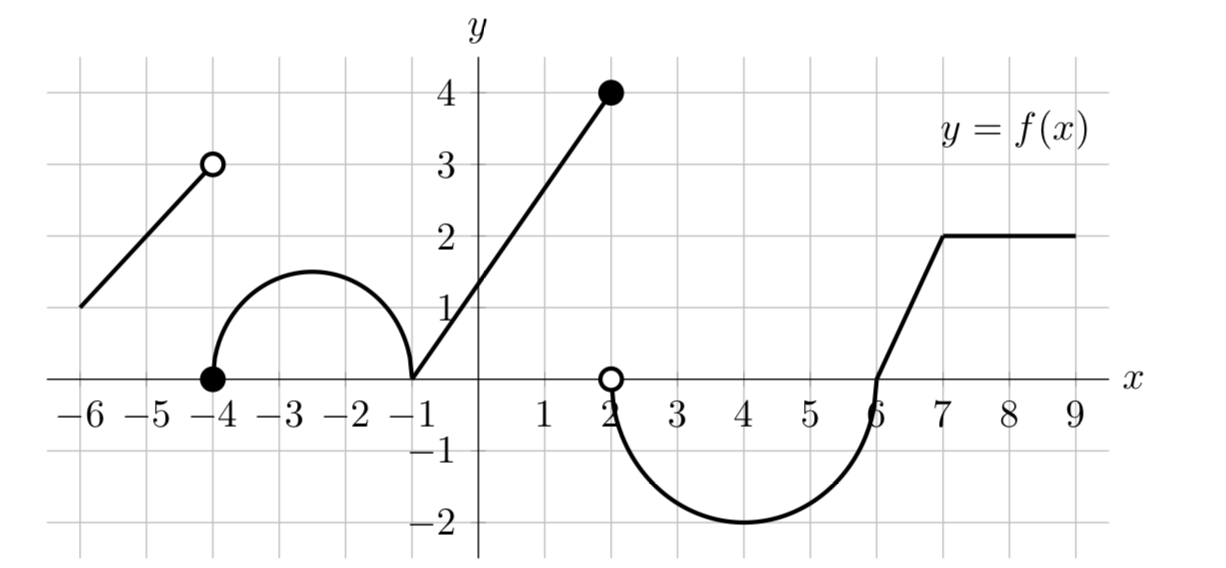
\includegraphics[scale=0.5]{graph1}
\end{center}
Use the graph above to calculate the answers to the following questions. Give your answers as exact values. You do not need to show work. If any of the answers cannot be found with the information given, write \emph{nei}.
\begin{enumerate}[(a)]
	\item Find the average value of $f(x)$ on $[-4,2]$.
	\item Find the value of $\displaystyle\int_{4}^9 |f(z)| \, dz$.
	\item Find the value of $4 \leqslant T \leqslant 9$ such that $\displaystyle\int_{4}^T f(z) \, dz = 0$.
	\item Find the value of $\displaystyle\int_{-8}^{-7} f(x+2)+1 \,\, dx$.
\end{enumerate}
\begin{solution}
  See \href{https://dhsp.math.lsa.umich.edu/exams/115exam3/w17/s2.pdf}{https://dhsp.math.lsa.umich.edu/exams/115exam3/w17/s2.pdf}
\end{solution}
\question (Winter 2013 Final Exam) % problem 9e 
	If $\displaystyle\int_{-1}^4 2 f(x) - 3 \, dx = -31,$ find $\displaystyle\int_{-1}^4 f(x)  \, dx$.
        \begin{solution}
          \[
            -31 = \int_{-1}^4 2 f(x) - 3 \, dx = 2\int_{-1}^4 f(x) dx -
            \int_{-1}^4 3 dx = 2 \int_{-1}^4 f(x) dx - 3(5) \implies
            \int_{-1}^4 f(x) dx = -8
          \]
        \end{solution}
\pagebreak
\question (Winter 2016 Final Exam)
A portion of the graph of a continuous function $g(x)$ is shown below. Assume that the area of the shaded region is 3 (as indicated on the graph), and note that $g(x)$ is piecewise linear for $2 < x < 6$.
\vspace{-1em}
\begin{center}
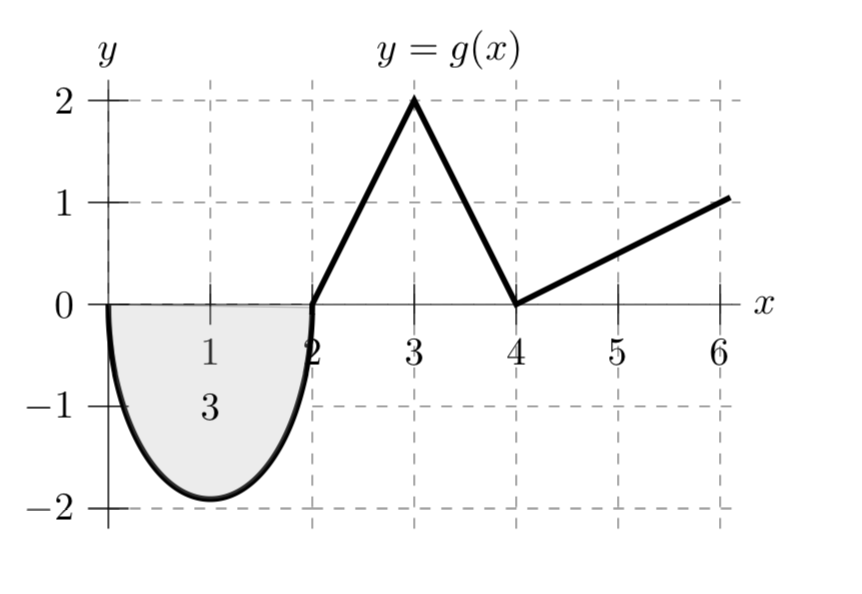
\includegraphics[scale=0.5]{graph2}
\end{center}
\begin{multicols}{2}
\begin{enumerate}[(a)]
	\item Find $\displaystyle\int_{0}^6 g(x) \, dx$.
	\item Find $\displaystyle\int_{0}^2 5 - 4g(x) \, dx$.	
	\item Suppose $C(x)=\ln(g(x))$. Find $C'(2.5).$
	\item Find $\displaystyle\int_{2}^4 g(x+2) - g(x-2) \, dx$.
	\end{enumerate}
	\end{multicols}
        \begin{solution}
          See \href{https://dhsp.math.lsa.umich.edu/exams/115exam3/w16/s6.pdf}{https://dhsp.math.lsa.umich.edu/exams/115exam3/w16/s6.pdf}
        \end{solution}
% \question (Winter 2014 Final Exam)
% 	One of the ways Captain Christina likes to relax in her retirement is to go for long walks around her neighborhood. She has noticed that early every Tuesday morning, a truck delivers butter to a local bakery famous for its cookie dough. Consider the following functions:
% 	\begin{itemize}
% 		\item Let $C(b)$ be the bakery's cost, in dollars, to buy b pounds of butter.
% 		\item Let $K(b)$ be the amount of cookie dough, in cups, the bakery makes from b pounds of butter.
% 		\item Let $u(t)$ be the instantaneous rate, in pounds per hour, at which butter is being unloaded $t$ hours after 4 am.
% 	\end{itemize}
% \begin{enumerate}[(a)]
% 	\item Interpret $K(C^{-1}(10)) = 20$ in the context of this problem.
% 	\item Interpret $\displaystyle\int_5^{12} K'(b) \, db = 40$ in the context of this problem.
% 	\item Give a single mathematical equality involving the derivative of C which supports the following claim:
% It costs the bakery approximately \$0.70 less to buy 14.8 pounds of butter than to buy 15 pounds of butter.
% 	\item Assume that $u(t)>0$ and $u'(t)<0$ for $0 \leqslant t \leqslant 4$ and that $u(2)=800$. Rank the following quantities in order from least to greatest.
% 	\begin{multicols}{4}
% 	\begin{enumerate}[I.]
% 	\item 0
% 	\item 800
% 	\item $\displaystyle\int_1^2 u(t) \, dt$
% 	\item $\displaystyle\int_2^3 u(t) \, dt$
% 	\end{enumerate} 
% 	\end{multicols}
% \end{enumerate}
      \question (Winter 2014 Final Exam) %problem 1
        The graph of a function $h(x)$ is shown below. The area of the shaded region $A$ is 4, and $h(x)$ is piecewise linear for $3 \leqslant x \leqslant 6$.
        \begin{center}
          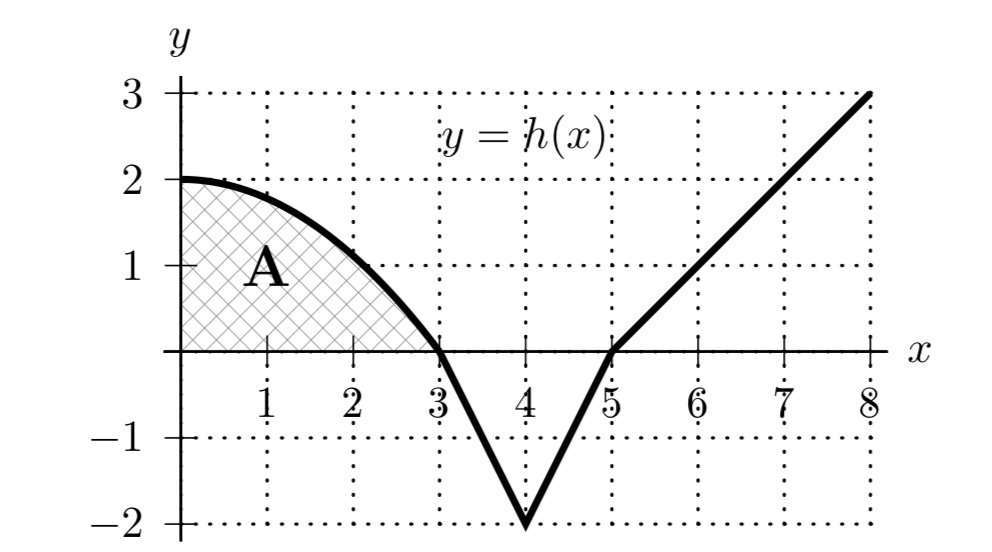
\includegraphics[scale=0.5]{graph3.png}
        \end{center}
Compute each of the following. If there is not enough information to compute a value exactly, write \emph{not enough info}.
\begin{enumerate}[(a)]
	\item Find $\displaystyle\int_0^3 h(t)+2 \, dt$.
	\item Find the average value of $h(x)$ on the interval $[0,4]$.
	\item Let $J(x) = \sin(\pi h(x))$. Find $J'(3.5)$.
	\item Let $g(x) = e^x$. Find $\displaystyle\int_6^7 g'(x)h(x) + g(x)h'(x) \, dt$.
\end{enumerate}
\begin{solution}
 See \href{https://dhsp.math.lsa.umich.edu/exams/115exam3/w14/s1.pdf}{https://dhsp.math.lsa.umich.edu/exams/115exam3/w14/s1.pdf}
\end{solution}
\end{questions}
  \end{document}
%%% Local Variables:
%%% mode: latex
%%% TeX-master: t
%%% End:
